\chapter{Diseño e implementación} % Main chapter title

\label{Chapter3} % Change X to a consecutive number; for referencing this chapter elsewhere, use \ref{ChapterX}

\definecolor{mygreen}{rgb}{0,0.6,0}
\definecolor{mygray}{rgb}{0.5,0.5,0.5}
\definecolor{mymauve}{rgb}{0.58,0,0.82}

%%%%%%%%%%%%%%%%%%%%%%%%%%%%%%%%%%%%%%%%%%%%%%%%%%%%%%%%%%%%%%%%%%%%%%%%%%%%%
% parámetros para configurar el formato del código en los entornos lstlisting
%%%%%%%%%%%%%%%%%%%%%%%%%%%%%%%%%%%%%%%%%%%%%%%%%%%%%%%%%%%%%%%%%%%%%%%%%%%%%
\lstset{ %
  backgroundcolor=\color{white},   % choose the background color; you must add \usepackage{color} or \usepackage{xcolor}
  basicstyle=\footnotesize,        % the size of the fonts that are used for the code
  breakatwhitespace=false,         % sets if automatic breaks should only happen at whitespace
  breaklines=true,                 % sets automatic line breaking
  captionpos=b,                    % sets the caption-position to bottom
  commentstyle=\color{mygreen},    % comment style
  deletekeywords={...},            % if you want to delete keywords from the given language
  %escapeinside={\%*}{*)},          % if you want to add LaTeX within your code
  %extendedchars=true,              % lets you use non-ASCII characters; for 8-bits encodings only, does not work with UTF-8
  %frame=single,	                % adds a frame around the code
  keepspaces=true,                 % keeps spaces in text, useful for keeping indentation of code (possibly needs columns=flexible)
  keywordstyle=\color{blue},       % keyword style
  language=[ANSI]C,                % the language of the code
  %otherkeywords={*,...},           % if you want to add more keywords to the set
  numbers=left,                    % where to put the line-numbers; possible values are (none, left, right)
  numbersep=5pt,                   % how far the line-numbers are from the code
  numberstyle=\tiny\color{mygray}, % the style that is used for the line-numbers
  rulecolor=\color{black},         % if not set, the frame-color may be changed on line-breaks within not-black text (e.g. comments (green here))
  showspaces=false,                % show spaces everywhere adding particular underscores; it overrides 'showstringspaces'
  showstringspaces=false,          % underline spaces within strings only
  showtabs=false,                  % show tabs within strings adding particular underscores
  stepnumber=1,                    % the step between two line-numbers. If it's 1, each line will be numbered
  stringstyle=\color{mymauve},     % string literal style
  tabsize=2,	                   % sets default tabsize to 2 spaces
  title=\lstname,                  % show the filename of files included with \lstinputlisting; also try caption instead of title
  morecomment=[s]{/*}{*/}
}

%----------------------------------------------------------------------------------------
\section{MTCNN con TensorFlow y TensorFlow Lite}
Como se explicó en el capitulo \ref{Chapter1}, el objetivo principal de este trabajo es detectar rostros humanos con ayuda de algoritmos de AI. Para esto se deben obtener imagenes digitales con ayuda de una camara, procesarlas y utilizarlas como entrada de una red de modelos de DL capaces de realizar la tarea de deteccion facial. Esta red de modelos de DL fue descrita en el capitulo \ref{Chapter2} y se denomina MTCNN.

Para implementar MTCNN adecuadamente no basta con alimentar P-Net con las imagenes obtenidas por la camara, R-Net con las ventanas candidatas de P-Net y O-Net con las ventanas candidatas de R-Net. Los datos de entrada de cada uno de los modelos de MTCNN deben ser procesados para conseguir el mejor resultado posible, como se muestra en el diagrama de la figura \ref{fig:mtcnn_npipe}.

\begin{figure}[h]
	\centering
	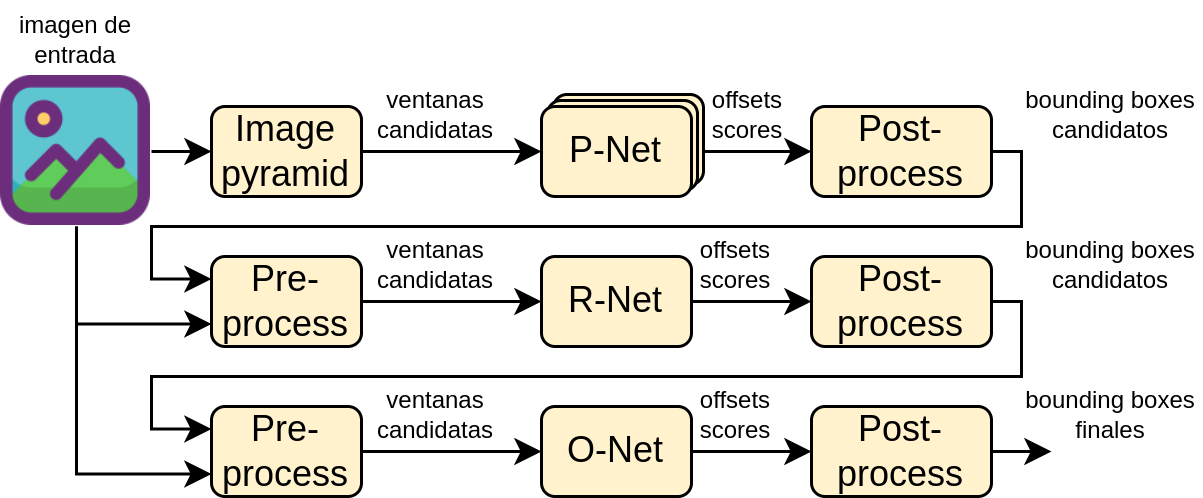
\includegraphics[scale=0.3]{./Figures/mtcnn_npipe.png}
	\caption{\textit{Pipeline} detallado de MTCNN.}
	\label{fig:mtcnn_npipe}
\end{figure}

El diagrama de la figura \ref{fig:mtcnn_npipe} muestra el \textit{pipeline} detallado de la red MTCNN, donde se pueden observar varios bloques de procesamiento, estos son:

\begin{itemize}
	\item \textit{Image pyramid}: genera a partir de la imagen de entrada otras imágenes de escalas inferiores, lo que permite detectar objetos de distintos tamaños. Cada nivel de escala se obtiene mediante la reducción de la escala anterior, por lo que las imágenes en niveles superiores tienen una escala mas baja que las imagenes en niveles inferiores. Después de generadas las imágenes escaladas requeridas de la imagen de entrada estas sirven para alimentar P-Net y así detectar rostros de distintos tamaños.

	\item \textit{Post-process}: en este bloque se procesan los datos de salida generados por P-Net, R-Net y O-Net. El primer subbloque realiza la operación de NMS para reducir la cantidad de ventanas candidatas que tienen solapmiento entre ellas. El segundo subbloque aplica un proceso de calibración que utiliza los \textit{offsets} generados por los modelos para determinar de manera mas precisa las coordenadas de las ventanas candidatas. Finalmente el último subbloque corrige las coordenadas de las ventanas candidatas para que posean dimensiones cuadradas y estén dentro de los límites de la imagen original.
	\begin{figure}[h]
		\centering
		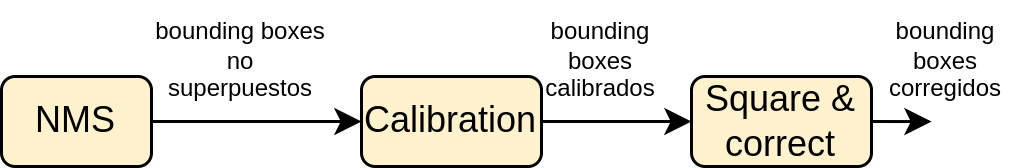
\includegraphics[scale=0.35]{./Figures/mtcnn_postprocess.png}
		\caption{Bloque de postprocesamiento.}
		\label{fig:mtcnn_postprocess}
	\end{figure}
	
	\item \textit{Pre-process}: tiene la función de procesar los datos de entrada para las redes R-Net y O-Net. El primer subbloque genera recortes de la imagen original en función de las coordenadas obtenidas del bloque \textit{post-process}. En el segundo subbloque las imágenes recortadas de entrada son redimensionadas con dimensiones de 24x24 px y 48x48 px, para alimentar R-Net y O-Net respectivamente.`
	\begin{figure}[h]
		\centering
		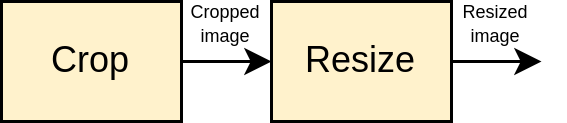
\includegraphics[scale=0.35]{./Figures/mtcnn_preprocess.png}
		\caption{Bloque de preprocesamiento.}
		\label{fig:mtcnn_preprocess}
	\end{figure}

\end{itemize}

P-Net, R-Net y O-Net fueron creados con ayuda de la biblioteca para redes neuronales Keras, que es parte del \textit{core} de TensorFlow, de acuerdo con lo expuesto en \cite{mtcnn_info}. Con las arquitecturas definidas de los modelos el siguiente paso natural en el desarrollo deberia haber sido su entrenamiento con uno o varios \textit{datasets}, pero al ser MTCNN tan popular en el ambito de deteccion facial se pudieron encontrar archivos de tipo HDF (\textit{Hierarchical Data Format}, Formato de Datos Jerárquicos) que contenian los \textit{weights} resultantes de un proceso de entrenamiento anterior. En el siguiente fragmento de codigo se puede observar el código utilizado para crear O-Net.

Para que los modelos obtenidos pudieran ser ejecutados en el hardware objetivo de este trabajo, tuvieron que ser convertidos a un formato más liviano y eficiente llamado TensorFlow Lite. El conversor de TensorFlow Lite toma un modelo de TensorFlow y genera un moelo de TensorFlow Lite cuya extensión de archivo es .tflite. La conversión puede seguir 2 caminos según como sean evaluados los modelos de TensorFlow, en la figura \ref{fig:tf2tflite_workflow} se observa el flujo de trabajo del conversor.

\begin{figure}[h]
	\centering
	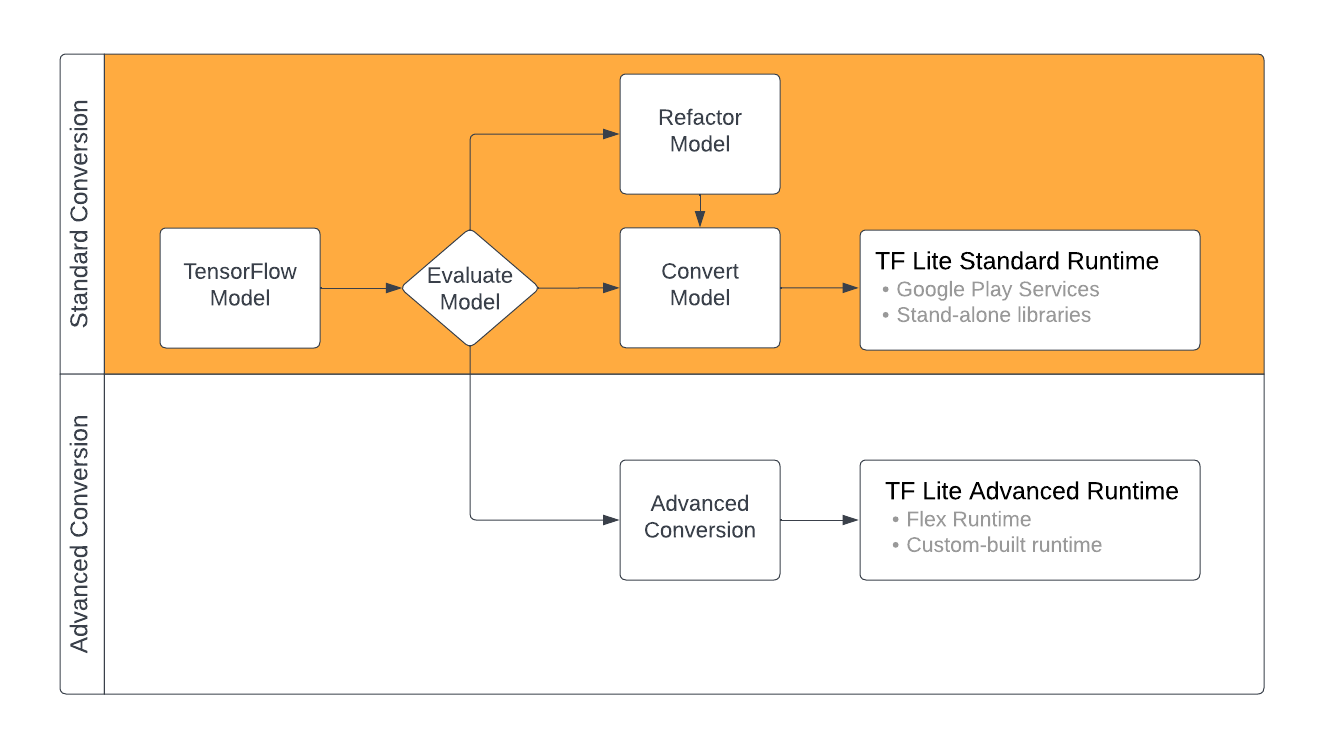
\includegraphics[scale=0.6]{./Figures/tf_convert_workflow_diag.png}
	\caption{Diagrama de flujo de trabajo para la conversion\protect\footnotemark.}
	\label{fig:tf2tflite_workflow}
\end{figure}
\footnotetext{Imagen tomada de: \url{https://www.tensorflow.org/lite/models/convert/}}

Gracias a que todos los operadores utilizados en los modelos de TensorFlow eran compatibles con los operadores de TensorFlow Lite se realizó una conversión estandar, lo que posteriormente facilitó su implementación en el hardware destino.

Durante el proceso de conversión se se aplicaron optimizaciones que responden a una necesidad de reducir aún más el tamaño y la latencia de los modelos. Se realizó una optmización por cuantización, que se refiere a la reducción de la precisión de los numeros usados para representar los parametros de los modelos, los cuales por defecto son flotantes de 32 bits. Las opciones de cuantización para los modelos se tomaron del diagrama de la figura \ref{fig:tf_quantization_tree}.

\begin{figure}[h]
	\centering
	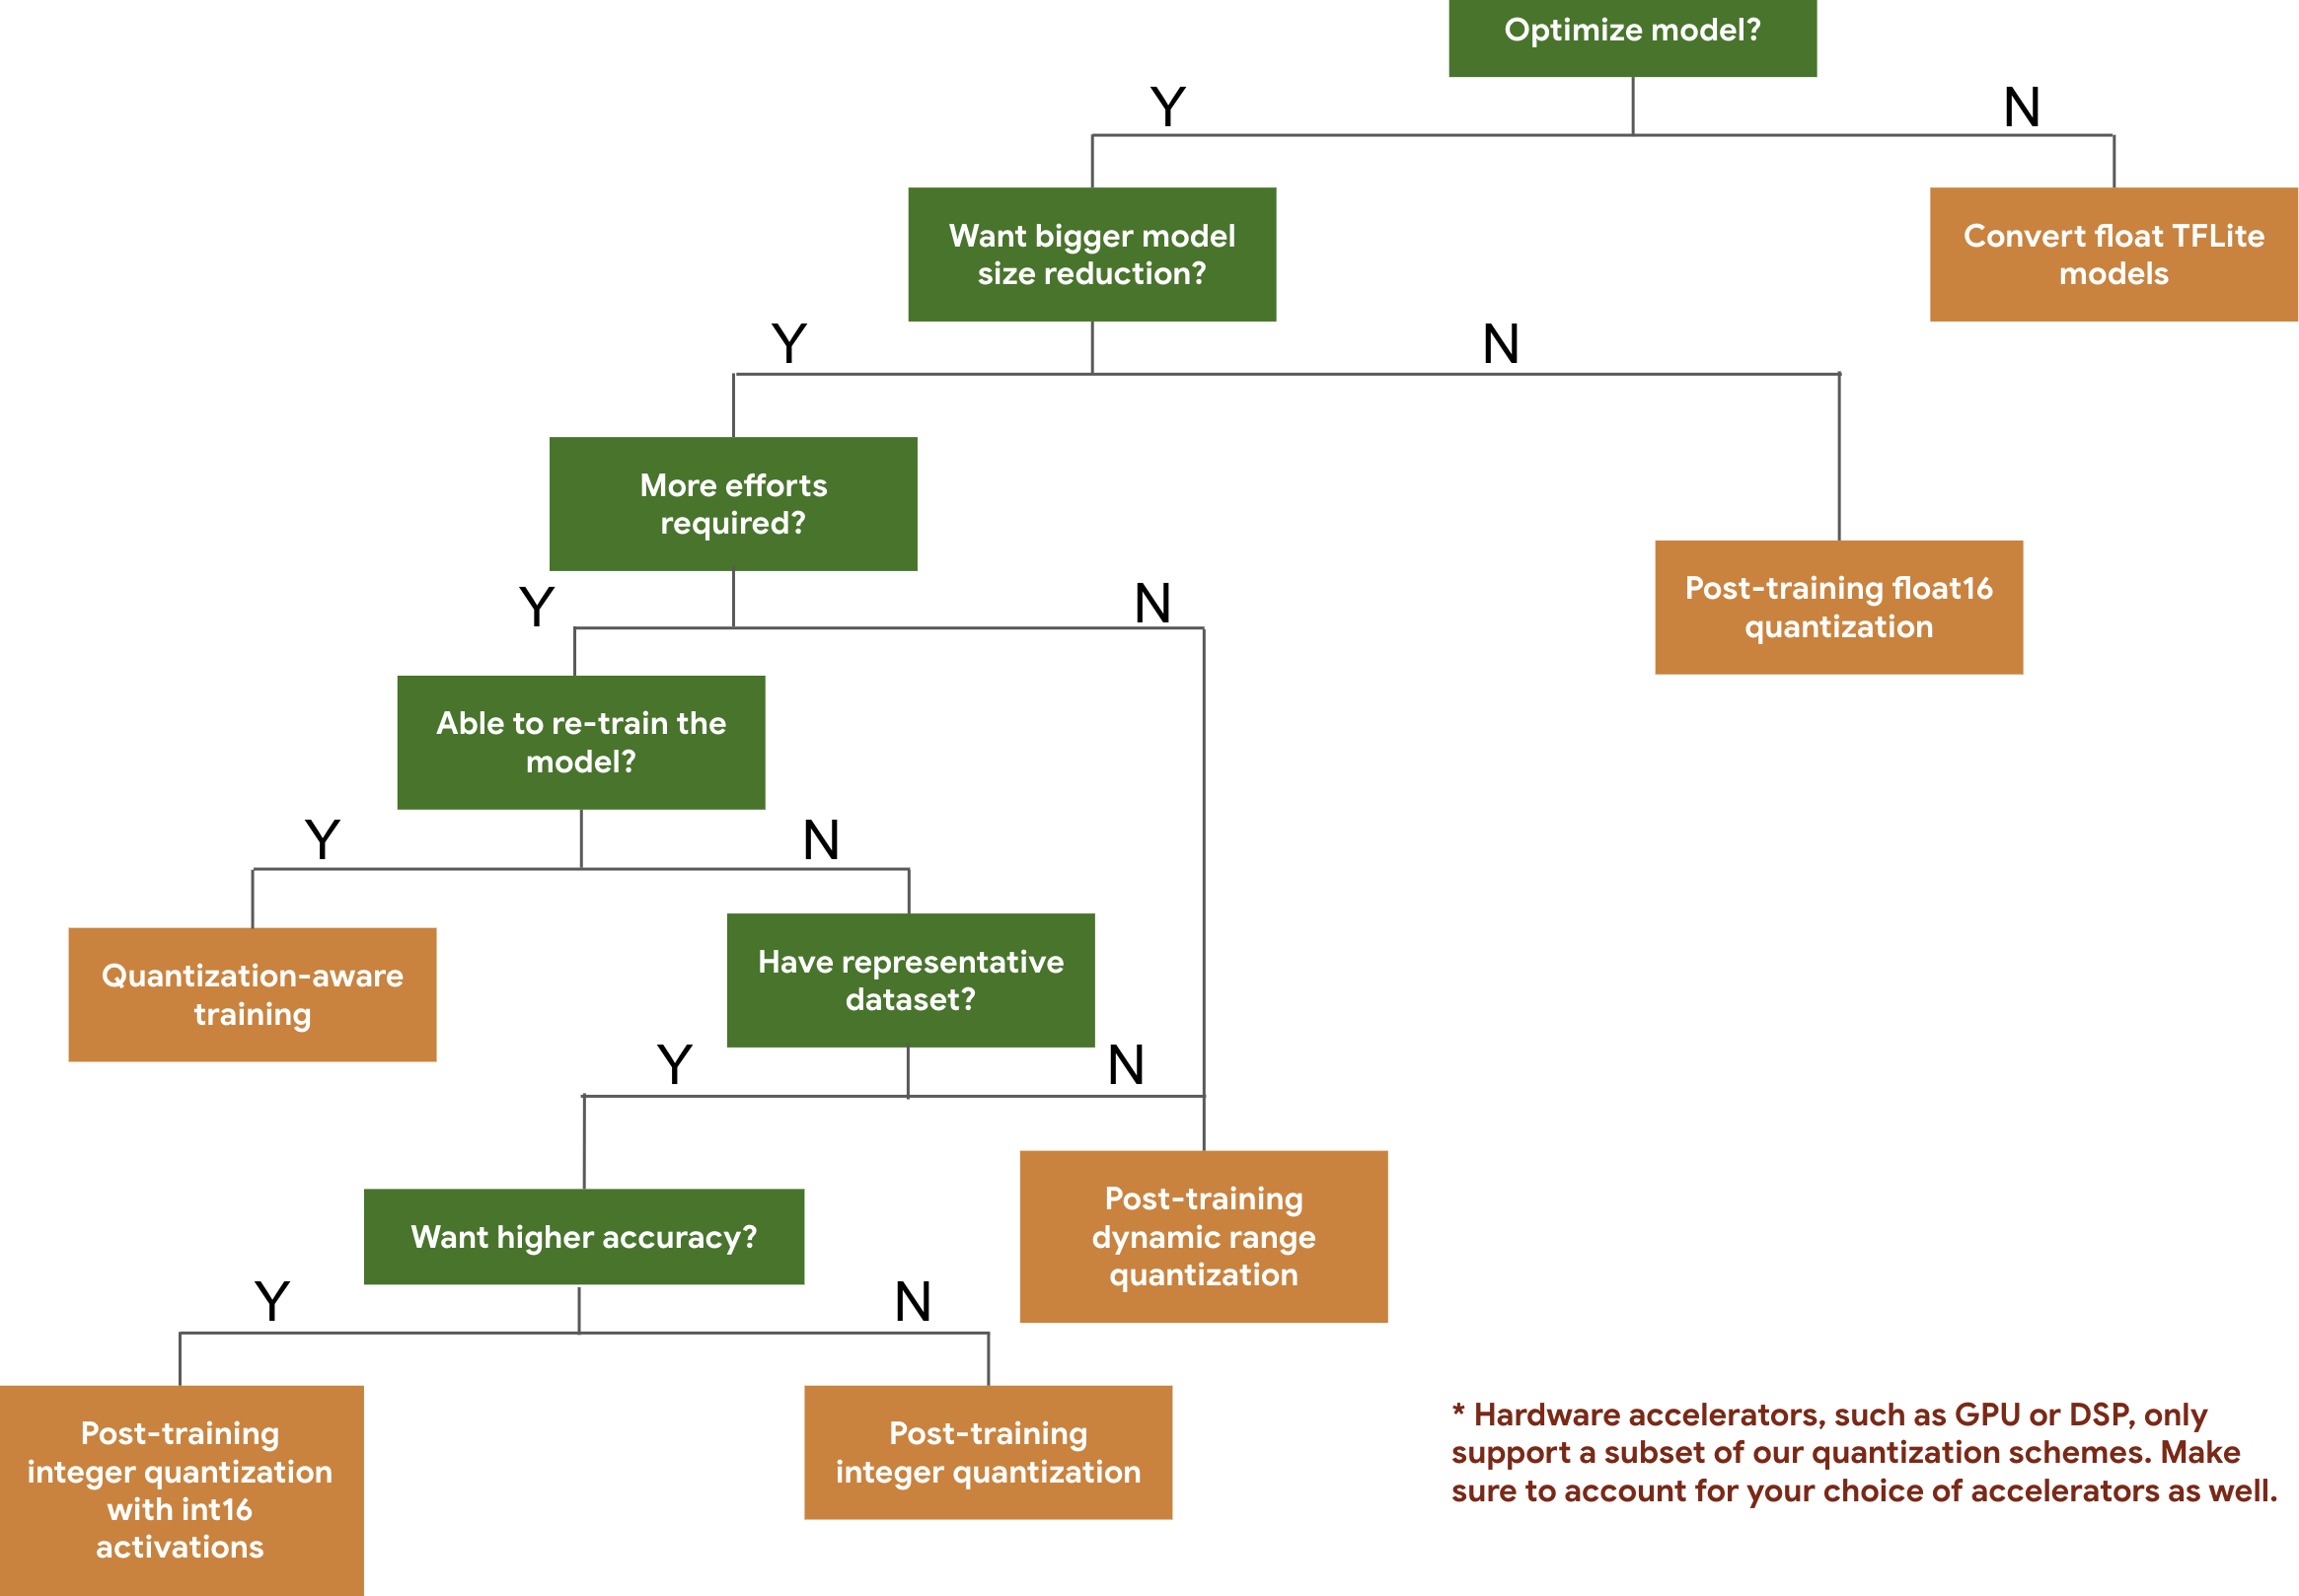
\includegraphics[scale=0.3]{./Figures/tf_quantization_decision_tree.png}
	\caption{Diagrama de árbol de decisiones para el proceso de cuantización\protect\footnotemark.}
	\label{fig:tf_quantization_tree}
\end{figure}
\footnotetext{Imagen tomada de: \url{https://www.tensorflow.org/lite/performance/model_optimization}}

La cuantizacion utilizada para los modelos fue \textit{full integer quantization}, que reduce los picos de memoria utilzados y asegura la compatibilidad con dispositivos de hardware que no pueden utilizar punto flotante. Para este tipo de cuantización se necesito crear un \textit{dataset} representativo, compuesto por un pequeno subconjunto (entre 100 a 500 muestras) del \textit{dataset} de entrenamiento. En ... se expone el codigo utilizado para la conversión de los modelos al formato TensorFlow Lite con cuantización a 8 bits.

La tabla \ref{tab:models_comp} muestra las diferencias entre los tamaños y latencias obtenidas de los modelos de TensorFlow, TensorFlow Lite sin quantización y TensorFlow Lite con cuantizacion a 8 bits.

\begin{table}[h]
	\centering
	\caption[Modelos comparativa]{Tabla comparativa de los modelos obtenidos}
	\begin{tabular}{lcc}   
		\toprule
		\textbf{TensorFlow} & \textbf{TensorFlow Lite} & \textbf{TensorFlow Lite int8} \\
		\midrule
		Tamaño (bytes) & 2 V a 15 V & x \\
		Latencia (ms) & 2 V a 15 V & x \\
		\bottomrule
		\hline
	\end{tabular}
	\label{tab:models_comp}
\end{table}

Todo el código para la obtención de los modelos hasta aquí expuesto, las funciones del \textit{pipeline}, las pruebas realizadas a los modelos y el despliegue de estos en el SoC ESP32-S3, se encuentra disponible en el repositorio de acceso público \cite{mtcnn_repo}.

%----------------------------------------------------------------------------------------
\section{Hardware}
\subsection{Sensor de movimiento}
\subsection{•}

%----------------------------------------------------------------------------------------
\section{Firmware}


\subsection{Cámara}
\subsection{MTCNN}
\subsection{Wi-Fi}
\subsection{MQTT y TLS}
\subsection{Sensor de movimiento}
\subsection{Bajo consumo}

%----------------------------------------------------------------------------------------
\section{Servicios en la nube}
\subsection{AWS IoT Core}
\subsection{AWS TimeStream}
\subsection{Grafana}




